\documentclass{article}
\usepackage[margin=1in]{geometry}
\usepackage{amsmath,amsthm,amssymb}
\usepackage{bbm,enumerate,mathtools}
\usepackage{tikz,pgfplots}
\usepackage{chessboard}
\usepackage[hidelinks]{hyperref}
\usepackage{multicol} % Problem 35

\newenvironment{question}{\begin{trivlist}\item[\textbf{Question.}]}{\end{trivlist}}
\newenvironment{note}{\begin{trivlist}\item[\textbf{Note.}]}{\end{trivlist}}
\newenvironment{references}{\begin{trivlist}\item[\textbf{References.}]}{\end{trivlist}}
\newenvironment{related}{\begin{trivlist}\item[\textbf{Related.}]\end{trivlist}\begin{enumerate}}{\end{enumerate}}


\begin{document}
  Let a ``popsicle stick weave'' be a configuration of lines segments, called ``sticks'', such that
  \begin{enumerate}[(1)]
    \item every stick has at least two sticks above it and one below or
      two sticks above and one below, and
    \item the removal of any stick results in a configuration that violates (1).
  \end{enumerate}

\begin{figure}[!h]
  \centering
  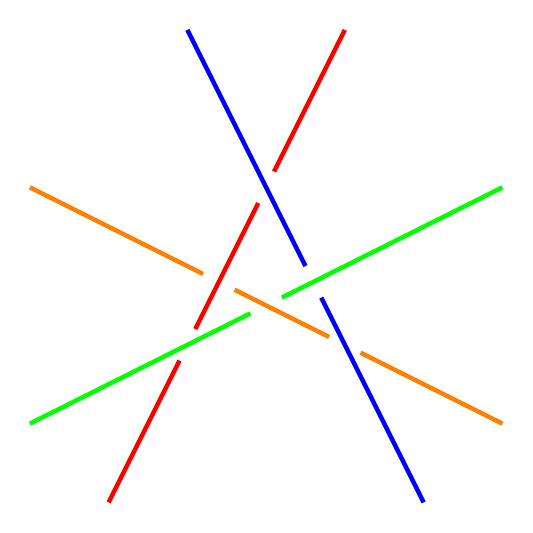
\begin{tikzpicture}
    % red(x) = 2x - 2
    \draw[ultra thick, red] (1,0) -- (1.9, 1.8);
    \draw[ultra thick, red] (2.1, 2.2) -- (2.9,3.8);
    \draw[ultra thick, red] (3.1,4.2) -- (4,6);
    % blue(x) = -2x + 10
    \draw[ultra thick, blue] (5,0) -- (3.7,2.6);
    \draw[ultra thick, blue] (3.5,3) -- (2,6);
    % green(x) = (1/2)x + 1
    \draw[ultra thick, green] (0,1) -- (2.8,2.4);
    \draw[ultra thick, green] (3.2,2.6) -- (6,4);
    % orange(x) = (-1/2)x + 4
    \draw[ultra thick, orange] (0,4) -- (2.2,2.9);
    \draw[ultra thick, orange] (2.6,2.7) -- (3.8,2.1);
    \draw[ultra thick, orange] (4.2,1.9) -- (6,1);
  \end{tikzpicture}
  \caption{The unique example of a 4 stick crossing (up to reflection)}
\end{figure}

\begin{question}
  How many distinct popsicle stick weaves exist for $n$ sticks?
\end{question}

\begin{related}
  \item What if the sticks are only allowed to touch three other sticks?
  \item What if the sticks are another geometric object (e.g. semicircles)?
\end{related}
\end{document}
